\section*{\huge \textcolor{Red}{ Decision Boundary } \small \textit{ Ranh giới quyết định } }
Tham khảo: \footnote{ \url{https://developers.google.com/machine-learning/glossary#decision-Boundary} }
\subsection*{Định nghĩa:}
Ranh giới quyết định là đường, mặt phẳng hay siêu mặt phẳng giúp phân chia vùng của các cụm (cluster) dữ liệu trong không gian.
Trong 1 bài toán phân loại có thể cho nhiều ranh giới quyết định tương ứng với nhiều lớp khác nhau.
\begin{{figure}}[!h]
	\centering
	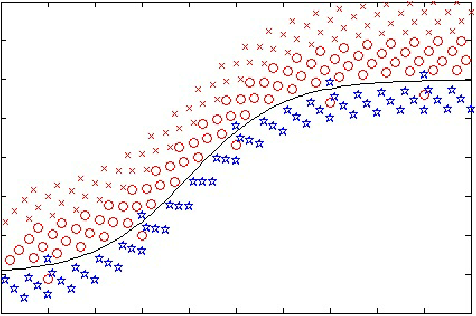
\includegraphics[width=0.4\linewidth]{ figures/D_Decision_boundary.png }
\label{fig:decision boundary_1}
\end{figure}

\section*{\huge \textcolor{Red}{ Digital Image } \small \textit{ Ảnh số } }
\subsection*{Định nghĩa:}
Ảnh số là khái niệm thường dùng trong phân tích và xử lý hình ảnh, được định nghĩa là một ma trận các điểm ảnh với các giá trị dùng để mô tả ảnh gần với ảnh thật.
\begin{{figure}}[!h]
	\centering
	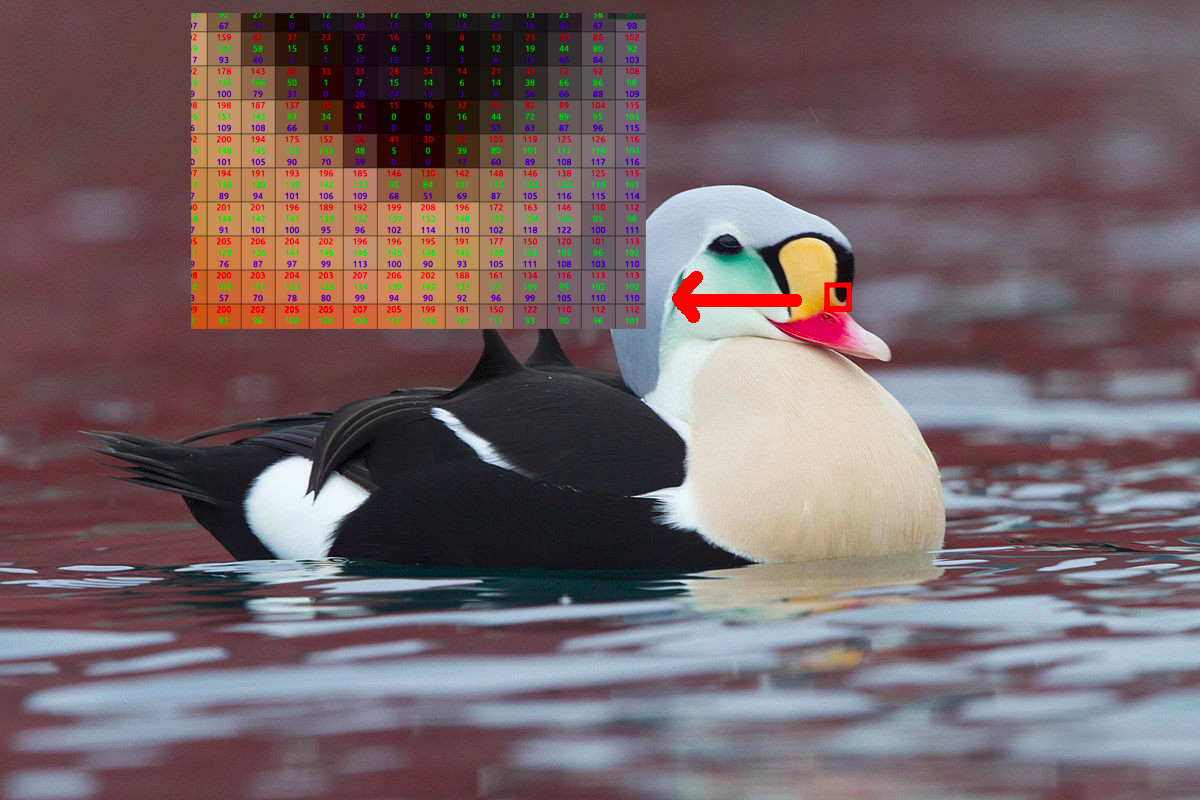
\includegraphics[width=0.75\linewidth]{ figures/D_Digital_Image_CPD_N1.png }
\label{fig:digital image_1}
\end{figure}
\subsection*{Mẹo nhỏ:}
Trong C/C++ và Python, thư viện \textit{{opencv}} thường được sử dụng để thao tác với ảnh số.

